% Beamer format
\documentclass[ignorenonframetext,9pt]{beamer}
\graphicspath{{figs/}}
% Article format
% \documentclass[10pt]{article}
% \usepackage{beamerarticle}

% Handout format
%  \documentclass[handout,ignorenonframetext]{beamer}

\mode<article>
{
  \usepackage{color}
  \usepackage{fullpage}
  \usepackage{geometry}
  \usepackage{pgf}
  \usepackage{hyperref}
}
%\usepackage[options]{natbib}
\mode<presentation>
{
%   \usetheme{PaloAlto}
%   \usetheme{Dresden}
%   \usetheme{Marburg}
%   \usetheme{Hannover}
%   \usetheme{Copenhagen}
%   \usetheme{Warsaw}
  \usetheme{default}
  \usecolortheme{whale}
  \setbeamercovered{transparent}
}

\mode<handout>
{
%%% In handout mode give the individual pages a light grey background
\setbeamercolor{background canvas}{bg=black!5}
%%% Put more than one frame on each page to save paper.
\usepackage{pgfpages} 
\pgfpagesuselayout{4 on 1}[letterpaper,border shrink=3mm, landscape]
% \pgfpagesuselayout{2 on 1}[letterpaper,border shrink=5mm, portrait]
% \setbeameroption{show notes}
}

% additional packages
\usepackage{graphicx}
\usepackage{caption}
\usepackage[utf8]{inputenc}
\usepackage[english]{babel}
\usepackage[normalem]{ulem}

% new commands

\newcommand{\xx}{\textbf{x}}
\newcommand{\yy}{\textbf{y}}
\newcommand{\ww}{\textbf{w}}
\newcommand{\cc}{\textbf{c}}
\newcommand{\CC}{\textbf{C}}
\newcommand{\dd}{\textbf{d}}
\newcommand{\NN}{\mathbb{N}}
\newcommand{\PP}{\mathcal{P}}
\newcommand{\RR}{\mathbb{R}}
\newcommand{\XX}{\mathcal{X}}
\newcommand{\YY}{\mathcal{Y}}
\newcommand{\mm}{\mathfrak{m}}

% use filled squares for itemizations
\setbeamertemplate{itemize items}[square]

% set the path to the figs directory
\newcommand{\figsdir}{./figs}

% set the command to the schedule import
\newcommand{\schedule}{\input{../schedule.tex}}

% set the bg color on boxes
% \setbeamercolor{bgcolor}{fg=white,bg=gray}

%%% Title Work
\title{\textbf{NOMA-SM for Cooperatively Enhancing V2V Transmissions  }\newline}
\author{\underline{Petru Lupascu}\newline}
\date{Thu., 19 Apr 2018\\ \flushright
\includegraphics[scale=0.18]{\figsdir/jub.png}}
\institute[JUB]{{\large{\textbf{Jacobs University Bremen}}} \\ \color{blue}{\href{mailto:p.lupascu@jacobs-university.de}{p.lupascu@jacobs-university.de}}}
%%

\begin{document}

%%% Frame 
% Title frame
\frame{
\maketitle
}
\section{Introduction}
\frame{
\frametitle{Motivation}
	\begin{itemize}
		\item In this paper the main focus is on developing a new scheme to accommodate the increasing demand for multi-media services and applications for the Vehicle to Vehicle communication system.
		\item The V2V system can be characterized by channel with high Spatial Correlation, we need a way to work around it. 
		\item Try to Amalgamate the robustness of Spatial Modulation against Spatially correlated channels and the Benefits of Non Orthogonal Multiple Access to deal with the effects of V2V channels and improve the Bandwidth efficiency.
	\end{itemize}
}


\frame{
\frametitle{}
	\begin{enumerate}
		\item Introduction
		\begin{enumerate}
			\item V2V System using massive MIMO
			\item Brief Introduction of the Spatial Modulation
			\item Intro to Noma %Angela does that , will do a short summary
		\end{enumerate}
		\item The Scheme
		\begin{itemize}
			\item[A.] NOMA SM 
			\item[B.] Massive MIMO Channel Model for V2V 
		\end{itemize}
	\item Capacity Analysis
	\item Power Allocation 
	\item Results %maybe simulation as well
	\end{enumerate}
}

\frame{
\frametitle{V2V System using massive MIMO}
\begin{itemize}
	\item In order to accommodate for the increase in the demand for multimedia services ew make use of the massive MIMO concept which offers ample Degrees of Freedom. But what is it ?
	\item Recall the $2x2$ MIMO scheme \\
	\flushleft\begin{figure}
	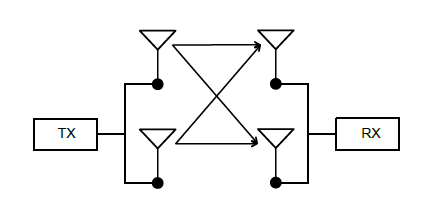
\includegraphics[scale=0.5]{MIMO22.png}\\
	\figurename{1. A 2x2 MIMO channel}
	\end{figure}
	$$\mathbf{ y = H \cdot s + w \hspace{0.3cm} \to \bar{y} = s+H^{-1}\cdot w}  \hspace{0.2cm},\hspace{0.2cm}  \boldsymbol{H} = \begin{bmatrix} h_{11} & h_{12} \\ h_{21} & h_{22}\end{bmatrix}$$
	$$\hat{s} = \underset{S^2}{min} \Bigg\lVert \boldsymbol{y} - \begin{bmatrix}
	h_{11}s_1 + h_{12}s_2 \\
	h_{21}s_1 + H_{22}s_2 \\
	\end{bmatrix} \Bigg\rVert^2 $$ 
	Consequently the channel has a degree of freedom of 2, Which can be generalized into n DOF for $n\times n$ MIMO	
\end{itemize}
	}

\frame{
\frametitle{From Single MIMO to Massive MIMO}
	\begin{itemize}
		\item The DOF can either be exploited for Diversity or Multiplexing, the combination of which lays the Basis of Massive MIMO.
		
		\begin{figure}
			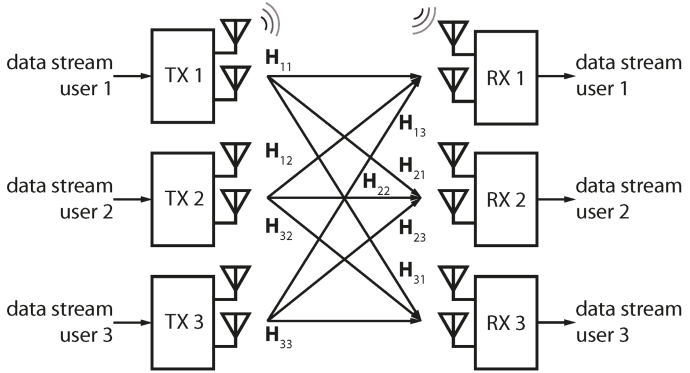
\includegraphics[scale=0.5]{MMIMOO.png}
			\figurename{2. Simple combination of the Diversity and Multiplexing}
		\end{figure}
	\item Massive MIMO uses the same concept but involves hundreds of Antenna. 
	\end{itemize}
}

\frame{
\frametitle{Spatial Modulation and Massive MIMO}
\begin{itemize}
	\item As a result , the Massive MIMO prvides an Increasing data rate, Increasing basic link signal to noise ratio and Channel hardening. 
	\item On the other hand it suffers from inter-antenna interference and in our Vehicular environment , from high Doppler propagation which aggravates the spatial correlation between antennas.
	\item In order to address some of these problems we make use of the Spatial Modulation which activates one transmit antenna at a time , thus reducing the IAI. As well SM-MIMO exhibits robustness against the spatial-temporally correlated channels.
\end{itemize}
}
\frame{
	\frametitle{So what is SM and how do we make use of it}
	\begin{figure}
		\centering 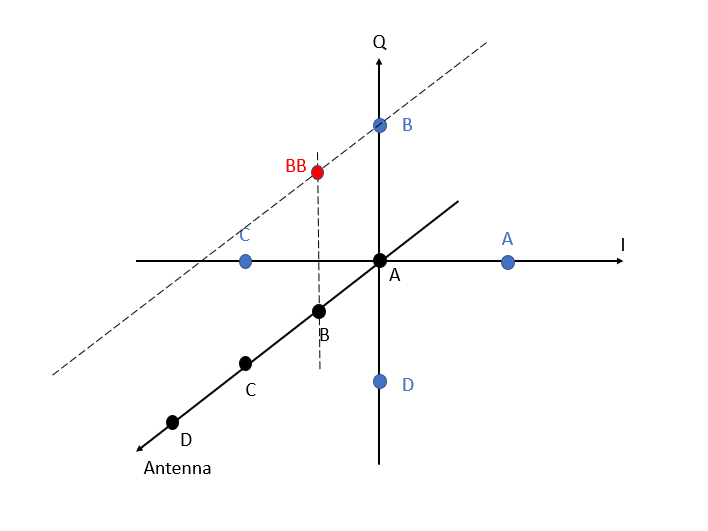
\includegraphics[scale=0.4]{SMexample.png} \\
		\centering \figurename{3. Encoding BB using SM}
	\end{figure} 
	\indent By activating one antenna per at a time MIMO-SM reduces significantly the Inter Antenna Interference and as well. 
}

\frame{
\frametitle{SM-MIMO model}
  \begin{itemize}
  	\item A system model of massive SM MIMO
  	\begin{figure}
  		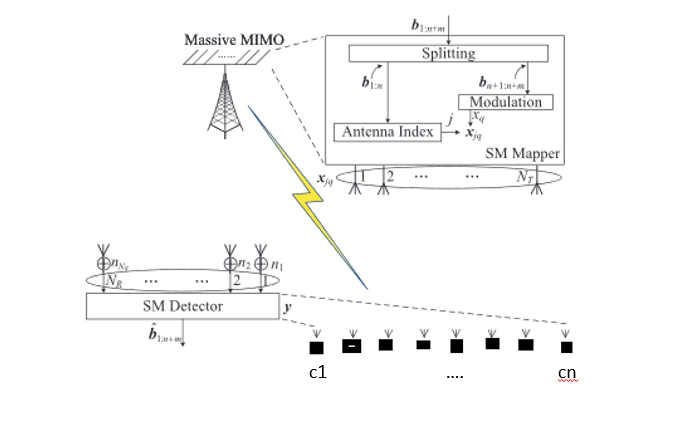
\includegraphics[scale=0.5]{SMMIMO.png}\\
  		\figurename{4. SM-MIMO model example}
  	\end{figure}
  \end{itemize}
}


\frame{
\frametitle{The idea of NOMA}
\begin{itemize}
	\item We already know from that the Orthogonal Multiple Access techniques allocate orthogonal resources in either time, frequency ir code in order to avoid or alleviate the IUI. \\
	\begin{figure}
		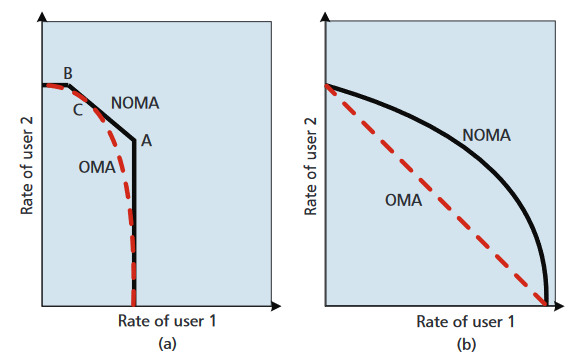
\includegraphics[scale=0.5]{NOMAOMA.png}\\
		\figurename{5. Channel capacity comparison of OMA and NOMA in an AWGN
			channel a) uplink b)downlink channel}
	\end{figure}
\end{itemize}
}

\frame{
\frametitle{NOMA via Power Domain Multiplexing}
	\begin{figure}
		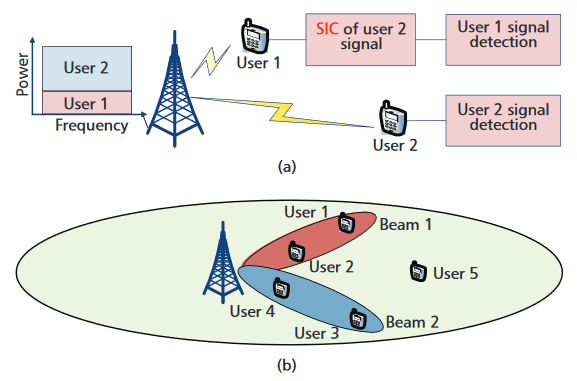
\includegraphics[scale=0.5]{NOMAPMUX.png}\\
		\figurename{6. NOMA via power domain multiplexing: a) basic
			NOMA with a SIC receiver b)NOMA in MIMO systems}
	\end{figure}
}

\frame{\frametitle{NOMA-SM-Proposed scheme}
	\begin{figure}
	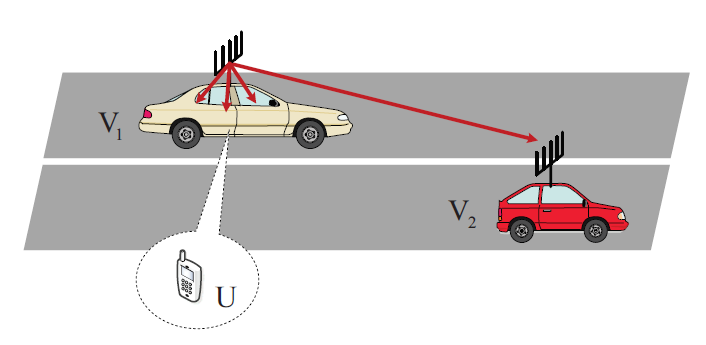
\includegraphics[scale=0.4]{car-scheme.png}\\
	\figurename{7. Vehicular transmission system, where
		the NOMA-SM strategy is applied}
	\end{figure}
	$\bullet$ $V_1$ and $V_2$ are in both in motion.
}

\frame{
\frametitle{ NOMA-SM-Proposed scheme}
	\begin{figure}
		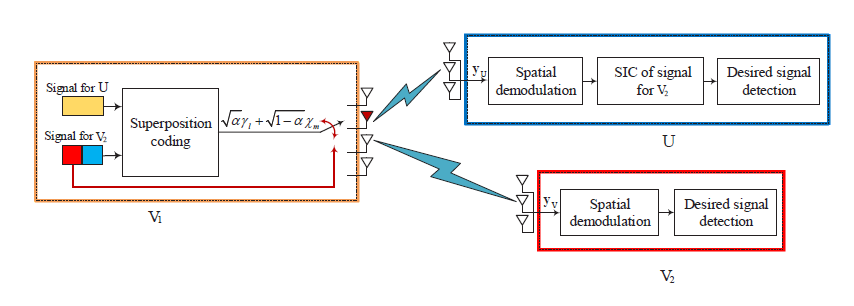
\includegraphics[scale=0.5]{schematic-diagram.png}\\
		\figurename{8. The Schematic Diagram}
	\end{figure}
	$\bullet$ $U$ and $V_2$ make their request to $V_1$ \\
	$\bullet$ Assume that $N_t$, $N_r$ and $N_u$ are omni directional antennas employed at each point. Consider as well the TA index$n_t \in \{1,...N_t\} $
}
\frame{
	\frametitle{Principles of NOMA-SM}
	\begin{itemize}
		\item The NOMA-SM is applied for both links: $V_1-V_2$ and $V_1-U$.
		\item At the transmitter 2 independent bit streams are prepared for transmissions.
		\item The bit stream for $V_2$ is partitioned into 2 parts. 
		\item First $\log_2(N_t)$ are used for TA activation. 
		\item Second $\log_2(M)$ bits destined for $V_2$ are combined with $\log_2(L)$ bits destined for $U$.
		\item Thus the modulated signal  $\sqrt{\alpha}\gamma_l+\sqrt{1-\alpha}\chi_m $   is transmitted by the  $n_t$ . Where: \\
		$\gamma_l$ and $\chi_m$ are  $l_{th}$ and $m_{th}$ symbol in L-ary and M-ary APM constellation \\ $\alpha$ is the power allocation factor.	

	\end{itemize}
}
\frame{\frametitle{Principles of NOMA-SM}
	\begin{itemize}
		\item The modulated symbol is satisfying $ \mathbb{E}(|\gamma_l|) = \mathbb{E}(|\chi_m|) = E_s $  - both constellations should have the same average energy per symbol at the receiver. 
		\item According to the NOMA principle $(1-\alpha)E_s > \alpha E_s$ which guarantees  $0<\alpha < 0.5 $
		\item As a result $log_2(N_tML)$ bits identifies the active TA $n_t$
		\item Thus the NOMA-SM super symbol:\\			
		 $ \boldsymbol{x} = \boldsymbol{e}_{n_t}( \sqrt{\alpha}\gamma_l+\sqrt{1-\alpha}\chi_m  )$ \\
		  $n_t$ is activated while $N_t-1$ TA are deactivated.
	\end{itemize}
}

\frame{
\frametitle{Principles of NOMA-SM}
\begin{itemize}
	\item Propagation between $V_1-U$ can be modeled by a frequency flat Rayleigh Channel which is applicable for the absence of a LOS.
	\item Define Channel Matrix $\boldsymbol{G} \in \mathbb{C}^{N_rxN_t}$ where all the entries are assumed to be independent identically distributed zero-mean Gaussian processes. $\mathcal{CN}(0,1)$.
	\item The received signal at U can be written as:
	$$ \boldsymbol{y}_U = \boldsymbol{g}_{n_t}\sqrt{\alpha}\gamma_l+\sqrt{1-\alpha}\chi_m + \boldsymbol{w_U} $$
\end{itemize}
}

\frame{
\frametitle{Principles of NOMA-SM}
	\begin{itemize}
		\item Since $V_2$ is further away the signal is subjected to Large Scale Fading which causes a power drop btw $V_1$ and $ V_2 $, call teh average power drop: $ p_0 $
		\item In similar fashion the received signal at $ V_2 $ can be written as: $$ \boldsymbol{y}_{V} = \sqrt{p_0} \boldsymbol{h}_{n_t}\sqrt{\alpha}\gamma_l+\sqrt{1-\alpha}\chi_m + \boldsymbol{w_V} $$
		\item Where: $ \boldsymbol{h}_{n_t} \in \mathbb{C}^{N_rx1} $ is the $ n_{th}  $ collum of the V2V channel matrix: $ \boldsymbol{H} \in \mathbb{C}^{N_rxN_t} $
		\item In both cases $ \boldsymbol{w}  $ denotes a complex AWGN vector with PDS $ \sigma_0^2 $ per entry.
	\end{itemize}
}



\frame{
\frametitle{Principles of NOMA-SM}
\begin{itemize}
	\item It is assumed that in the system both receivers have perfect synchronization in both time and frequency and Full channel state information is assumed to be avaiable at receiver.
	\item The corresponding ML are invoked according to: \\
	\centering 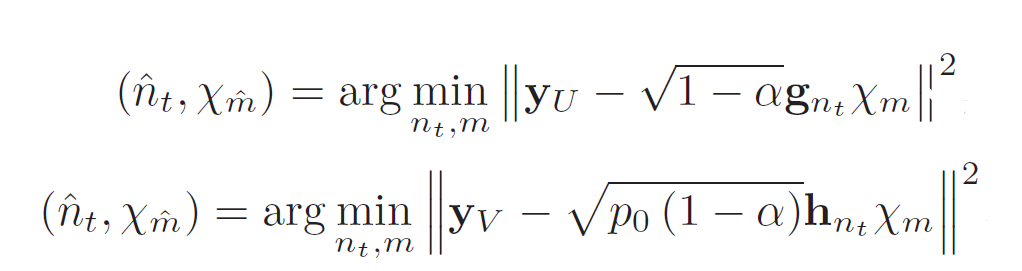
\includegraphics[scale=0.25]{MLdectors.png} \\
	\item Where both $ U $and $ V_2 $ have to detect the signal meant for $ V_{2} $. \\
	After eliminating the interference from $ (\hat{n}_t), \chi_m $ on $ \boldsymbol{y_U} $ U performs another ML detection to decode it's own symbol $ \gamma_l $.	
\end{itemize}
}

\frame{
	\frametitle{Massive MIMO Channel Model}
	\begin{itemize}
		\item The underline ideas of the V2V model  is that both Transmitter and Receiver are in motion and are being equipped woth low elevation antennas which results in different propagation delay. 
		\item The Rician channel moddel is being addopted for $ \boldsymbol{H}\in\mathbb{C}^{N_txN_r} $ which is given by: $$ \boldsymbol{H} = \sqrt{\dfrac{K}{K+1}}\boldsymbol{\bar{H}} + \sqrt{\dfrac{1}{K+1}}\boldsymbol{\tilde{H}}  $$
		Where: 
	    $ \boldsymbol{\bar{H}} $ is the fixed part related to the LOS component
		$ \boldsymbol{\tilde{H}} $ represents the variable part described by $ \boldsymbol{\tilde{H}} = \boldsymbol{\Sigma}^{1/2}_{r}\boldsymbol{\hat{H}} \boldsymbol{\Sigma}^{1/2}_{r} $ \\
		$ \boldsymbol{\Sigma}^{1/2}_{t} \in \mathbb{C}^{N_txN_t}$ and $ \boldsymbol{\Sigma}^{1/2}_{r} \in \mathbb{C}^{N_rxN_r} $ correlation matrices at V1 and V2 determined according to the Loyka exponential model: \\
		 $ [\boldsymbol{\Sigma}_t]_{q, \hat{q}} = k^{q-\hat{q}} $ and $ [\boldsymbol{\Sigma}_r]_{p, \hat{p}} = k^{p-\hat{p}} $ where: $ k_t $ and $ k_r $ are adjacent antenna correlation coefficients. \\
		$ \boldsymbol{\hat{H}} $ is the independent Rayleigh channel matrix entries of which $ \in \mathcal{CN} (0,1) $
		\item Lastly represent the temporal correlation as: $ \delta(\tau) = \mathbb{E}\{ \boldsymbol{\hat{H}(t)}\boldsymbol{\hat{H}(t+\tau)} \} $ \\
		$ \delta = 1 $ represents a quasi-static channel,  $ \delta < 1 $ - time varying channel. 
	\end{itemize}
}

\frame{
\frametitle{Capacity Analysis of the NOMA-SM system -of V2}
\begin{itemize}
	\item Recall that the message meant for $ V_2 $ is conveyed in both TA and signal domain spaces while the one for $ U $ only in the signal domain.
	\item Since transmit power for $ V_2 $ is larger, the interference from $ U $ can be treated as noise.
	\item Capacity of the instantaneous signal domain is given by: \\
	\centering 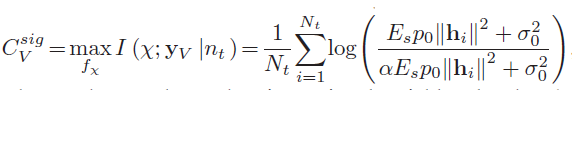
\includegraphics[scale=0.5]{capacityv2.png} \\
	$ \chi $ and $ f_\chi $ are the random symbol input and its PDF respectively. 
\end{itemize}

}

\frame{
	\frametitle{Capacity Analysis of the NOMA-SM system -of V2}
	\begin{itemize}
		\item At the same the mutual information conveyed in the TA domain can be represented as: \\
		\centering 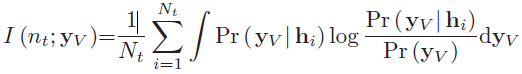
\includegraphics[scale=0.5]{tacapacity.png} \\
		Where: \\ 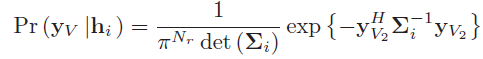
\includegraphics[scale=0.5]{prob1.png} \\
		in which: $ \boldsymbol{\Sigma}_i = \sigma^2_0\boldsymbol{I} + pE_s\boldsymbol{h}_i\boldsymbol{h}_i^H $ 
	\end{itemize}
	
	\centering \begin{LARGE}
		$ C_V = C_V^{sig} + I(n_t; \boldsymbol{y}_V) $
	\end{LARGE} \\	
}

\frame{
\frametitle{Capacity Analysis of the NOMA-SM system of U}
\begin{itemize}
	\item Opossite to $ V_2 $ , $ U $ can detect it's own signal only after removing the interference form $ V_2 $.
	\item As a result: \\
	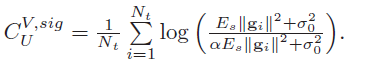
\includegraphics[scale=0.5]{capacityU.png} \\
	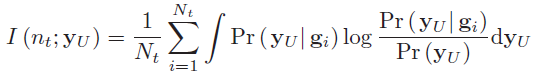
\includegraphics[scale=0.5]{tamiu.png} \\
	With: 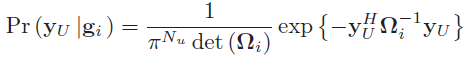
\includegraphics[scale=0.4]{prob2.png} where: $ \boldsymbol{\Omega}_i = \sigma^2_0\boldsymbol{I} + pE_s\boldsymbol{g}_i\boldsymbol{g}_i^H $ 
	\item As a result the instanteneus capacity of $ U $ to detect the signal of $ V_2 $ can be represented as: $$  C_U^{V} = C_U^{V,sig} + I(n_t; \boldsymbol{y}_U) $$
\end{itemize}
}

\frame{
\frametitle{Capacity Analysis of the NOMA-SM system of U}
  \begin{itemize}
  	\item It can bee seen that $ C_U^V > C_V $ since $ \vert\vert \boldsymbol{g}_i \vert\vert ^2 > p_0\vert\vert \boldsymbol{h}_i \vert\vert ^2$
  		\item Hence: \\
  	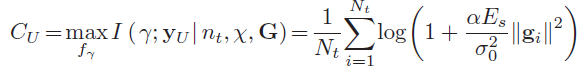
\includegraphics[scale=0.6]{capacityUfinal.png}\\
  	where: $ \gamma $ and $ f_\gamma $ are the random input signal and it's PDF. 
  	\item \textbf{The capacity of U to detect $ \gamma $ become achievable when $ f_{\gamma} $ is Gaussian.}
  \end{itemize}
}

\frame{
\frametitle{Power Allocation Optimization}
\begin{enumerate}
	\item The MI conveyed by the TA-domain cannot be readily formulated as a closed-form
	expression.
	\item In order to perform optimal power allocation we need an upper bound for the NOMA-SM capacity since power allocation
	optimization, which is capable of maximizing the capacity
	bound is considered, leading to the optimal solution.
\end{enumerate}
}

\frame{
	\frametitle{Upper Bound for NOMA-SM capacity}
	\begin{itemize}
		\item Instantaneous Capacity for $ V_2 $ can be expressed as : \\
			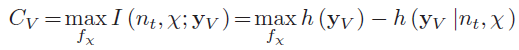
\includegraphics[scale=0.5]{diffev2.png} \\
			where" $  h(\cdot) $ represents the differential entropy and: \\
			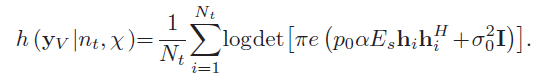
\includegraphics[scale=0.5]{diffev21.png} 
		\item MI $ I(n_t, \chi ;\boldsymbol{y}_V) $ is maximized if the vector $ \boldsymbol{y}_V $ is Gaussian-distributed with 0zero mean and a covariance as: $ \dfrac{p_0E_s}{N_t}\boldsymbol{H}\boldsymbol{H}^H + \sigma_0^2\boldsymbol{I} $. 
	\end{itemize}	
}

\frame{
\frametitle{Upper Bound for NOMA-SM capacity}
	\begin{itemize}
		\item Thus: $ h(\boldsymbol{y}_C) \leq log det(\pi e(\dfrac{p_0E_s}{N_t}\boldsymbol{H}\boldsymbol{H}^H + \sigma_0^2\boldsymbol{I}))$
		\item Hence the upper bound from the classical signal domain: \\
		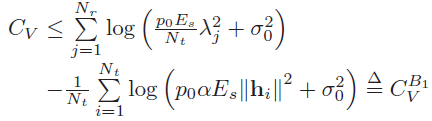
\includegraphics[scale=0.5]{upbcv1.png} \\
		where $ \lambda_j  $ is the j-th singular value of $ \boldsymbol{H} $ with $ j \in \{1,..,N_t\} $
	\end{itemize}
}

\frame{\frametitle{Upper Bound for NOMA-SM capacity}
\begin{itemize}
	\item Corollary the MI from TA is naturally bounded by $ I(n_t ; \boldsymbol{y}_V) \leq log(N_t) $
	\item As a consequence :\\
	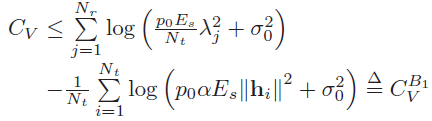
\includegraphics[scale=0.5]{upbcv1.png} 
\end{itemize}
}

\frame{
\frametitle{Upper Bound for NOMA-SM capacity}
$ \bullet $ Based on the above, a refined upper bound for the capacity of $ V_2 $ is represented as: 
\begin{Large}
	$ C_V^B = min(C_{V}^{B_1}, C_V^{B_2}) $ 
\end{Large} \\
	\begin{figure}
		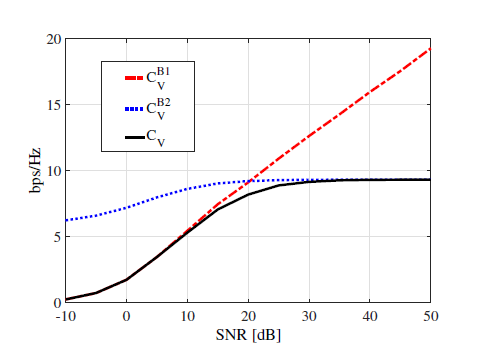
\includegraphics[scale=0.5]{capgraph.png}\\
		\figurename{9. Upper bound of the Capacity}
	\end{figure}
}

\frame{
	\frametitle{Power Allocation Optimization Scheme} 
	\begin{itemize}
		\item Taking into the account the QoS of the two receiver we define a minimum rate of $ V_2 $ and $ U $ as $ \tilde{C}_V $ and $ \tilde{C}_U $ \\
		\item Thus the optimization problem is constructed as: \\
		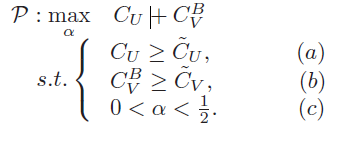
\includegraphics[scale=0.5]{optprob.png}
	\end{itemize}
}

\frame{
\frametitle{Power Allocation Optimization Scheme}
		\centering
		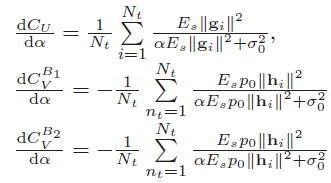
\includegraphics[scale=0.5]{optpder.png} \\
		 By satisfying (a) and (b) : \\
		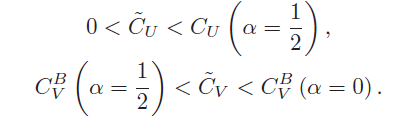
\includegraphics[scale=0.5]{optbd.png} \\
		Given which compactly rewrite the constraints of $ \mathcal{P} $ as: \\
		$ g^{-1}(\tilde{C}_U) < \alpha < f^{-1}(\tilde{C}_V) $ ; where $ g^{-1} $ and $ f^{-1}$ are the inverse function for $ C_U $ and $ C^B_V$.
	
}

\frame{
\frametitle{Power Allocation Optimization Scheme}
	To guarantee that the feasible set of $ \mathcal{P} $ is non-empty a further refined condition is given by: 
	$$ C_V^B(\alpha = 0.5) < \tilde{C}_V |< C_V^B[\alpha = g^{-1}(\tilde{C}_U)] $$
	Since  $ \vert\vert \boldsymbol{g}_i \vert\vert ^2 > p_0\vert\vert \boldsymbol{h}_i \vert\vert ^2$ is always true , derivative of $ (C_U+C_V^B) $ is always positive. \\
	Thus:
	$$ \alpha_{opt}^\mathcal{P} = f^{-1}(\tilde{C}_V) $$
}

\frame{
\frametitle{Power Allocation algorithm}
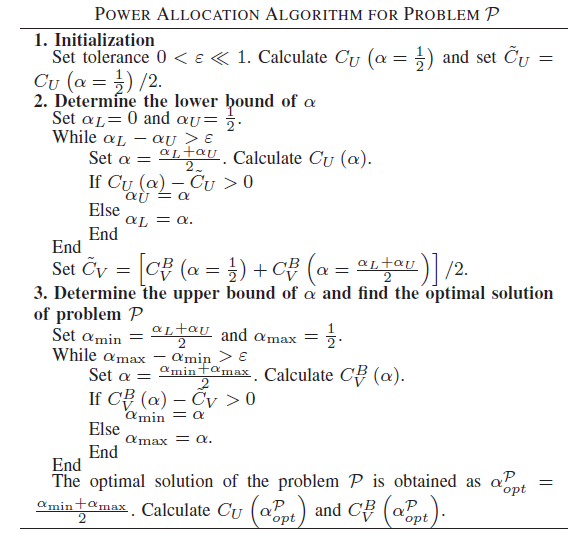
\includegraphics[scale=0.6]{optalgo.png}
}

\frame{
\frametitle{Results-Performance}
	\begin{figure}
	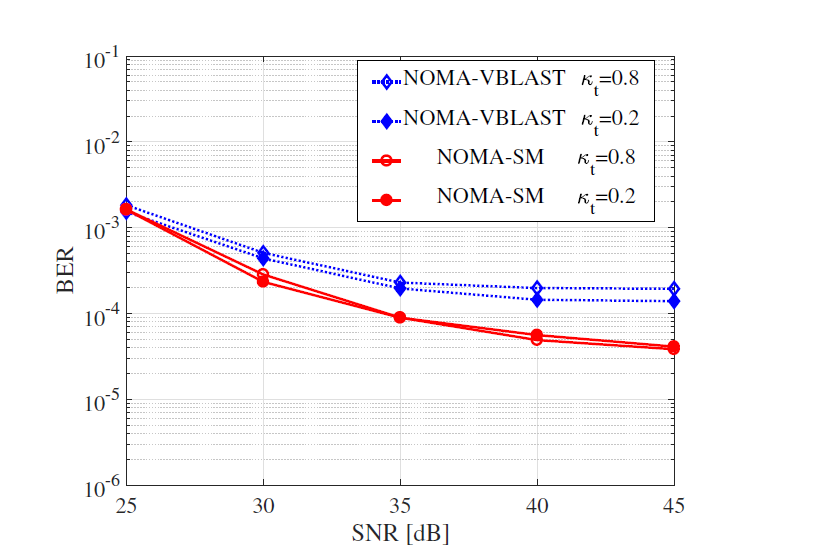
\includegraphics[scale=0.45]{result1.png}\\
	\figurename{10. BER comparisons with different adjacent antenna correlation
		coefficient at$V_1$, i.e.$k$, with fixed K = 0.2, $k_r$ = 0.5, $\delta$ = 1, and $\alpha$ = 0.001}
	\end{figure}
}

\frame{
	\frametitle{Results-Performance}
	\begin{figure}
		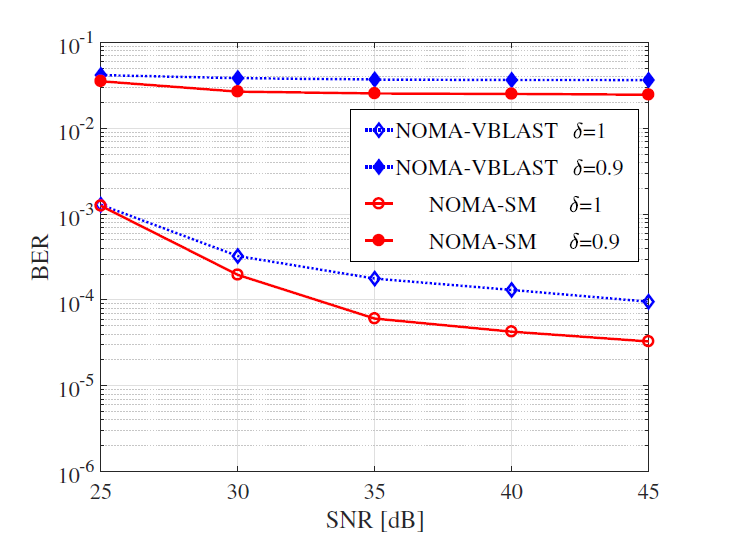
\includegraphics[scale=0.45]{result2.png}\\
		\figurename{11. BER comparisons with different temporal correlation coefficient $ \delta $ when $ K = 0.2 $, $ k_t = k_r = 0.5 $ and $ \alpha = 0.001 $ are fixed}
	\end{figure}
}

\frame{
	\frametitle{Results-Capacity}
	\begin{figure}
		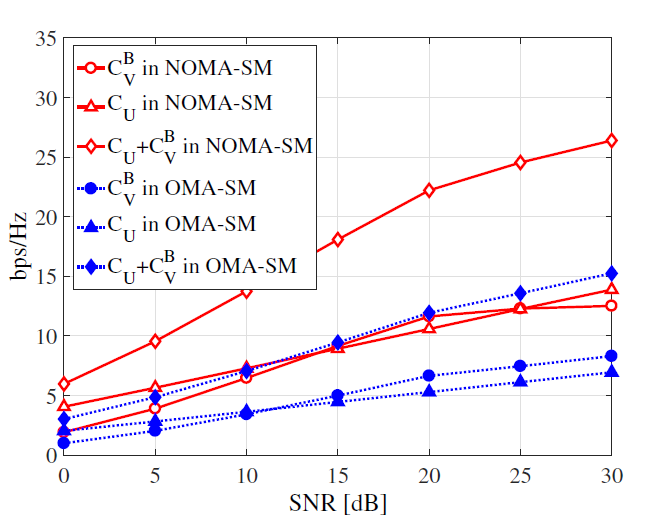
\includegraphics[scale=0.45]{result3.png}\\
		\figurename{12.Capacity Results with fixed power allocation$ \alpha= 0.01 $}
	\end{figure}
}

\frame{
	\frametitle{Results-Capacity}
	\begin{figure}
		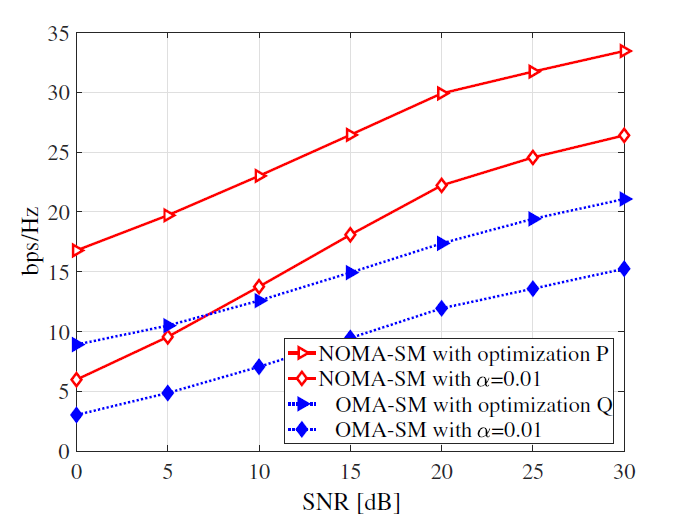
\includegraphics[scale=0.45]{result4.png}\\
		\figurename{12.Capacity Results with optimd power allocation}
	\end{figure}
}

\frame{
\frametitle{References}
\begin{enumerate}
	\item E.G. Larsson O. Edfors F. Tufvesson T.L. Marzetta "Massive MIMO for next generation wireless systems" IEEE Communications Magazine vol. 52 no. 2 pp. 186-195 Feb. 2014. 
	\item Y. Cui X. Fang "Performance analysis of massive spatial modulation MIMO in high-speed railway" IEEE Transactions on Vehicular Technology vol. 65 no. 11 pp. 8925-8932 Nov. 2016.  
	\item L. Dai B. Wang Y. Yuan S. Han C.I Z. Wang "Non-orthogonal multiple access for 5G: Solutions challenges opportunities and future research trends" IEEE Communciations Magazine vol. 53 no. 9 pp. 74-81 Sept. 2015. 
\end{enumerate}
}
%%%
%%%
\end{document}
